\documentclass[11pt,a4paper]{article}

% ============================================================================
% PACKAGES
% ============================================================================
\usepackage[utf8]{inputenc}
\usepackage[T1]{fontenc}
\usepackage{geometry}
\usepackage{graphicx}
\usepackage{booktabs}
\usepackage{amsmath}
\usepackage{amssymb}
\usepackage{hyperref}
\usepackage{xcolor}
\usepackage{listings}
\usepackage{float}
\usepackage{caption}
\usepackage{subcaption}
\usepackage{enumitem}
\usepackage{fancyhdr}
\usepackage{tikz}
\usepackage{pgfplots}
\usepackage{multicol}
\usepackage{algorithm}
\usepackage{algpseudocode}
\usepackage{longtable}
\usepackage{pifont}
\pgfplotsset{compat=1.17}

% ============================================================================
% PAGE SETUP
% ============================================================================
\geometry{margin=1in}
\setlength{\parindent}{0pt}
\setlength{\parskip}{0.5em}

% Header/Footer
\pagestyle{fancy}
\fancyhf{}
\rhead{MetaFam Knowledge Graph}
\lhead{Task 3: Rule Mining}
\rfoot{Page \thepage}

% Colors
\definecolor{codegreen}{rgb}{0,0.6,0}
\definecolor{codegray}{rgb}{0.5,0.5,0.5}
\definecolor{codepurple}{rgb}{0.58,0,0.82}
\definecolor{backcolour}{rgb}{0.95,0.95,0.92}
\definecolor{highconf}{HTML}{55A868}
\definecolor{medconf}{HTML}{F5A623}
\definecolor{lowconf}{HTML}{C44E52}

% Hyperref setup
\hypersetup{
    colorlinks=true,
    linkcolor=blue,
    filecolor=magenta,
    urlcolor=cyan,
}

% ============================================================================
% DOCUMENT
% ============================================================================
\begin{document}

% ----------------------------------------------------------------------------
% TITLE PAGE
% ----------------------------------------------------------------------------
\begin{titlepage}
    \centering
    \vspace*{2cm}
    
    {\Huge\bfseries MetaFam Knowledge Graph\\[0.5cm]Task 3: Rule Mining\par}
    
    \vspace{1.5cm}
    
    {\Large\textit{``Happiness can be found even in the darkest of times,\\if only one remembers to turn on the light''} --- Albus Dumbledore\par}
    
    \vspace{2cm}
    
    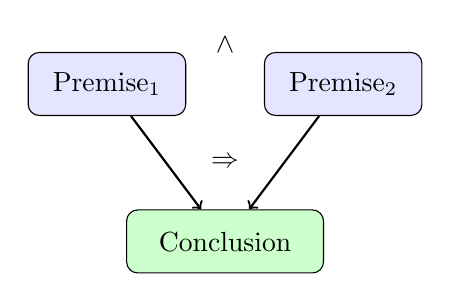
\begin{tikzpicture}
        % Horn clause visualization
        \node[draw, rounded corners, fill=blue!10, minimum width=2cm, minimum height=0.8cm] (p1) at (0,0) {Premise$_1$};
        \node[draw, rounded corners, fill=blue!10, minimum width=2cm, minimum height=0.8cm] (p2) at (3,0) {Premise$_2$};
        \node[draw, rounded corners, fill=green!20, minimum width=2.5cm, minimum height=0.8cm] (c) at (1.5,-2) {Conclusion};
        
        \draw[->, thick] (p1) -- (c);
        \draw[->, thick] (p2) -- (c);
        
        \node at (1.5, 0.5) {$\land$};
        \node at (1.5, -1) {$\Rightarrow$};
    \end{tikzpicture}
    
    \vspace{2cm}
    
    {\large Precog Research Task\\[0.3cm]
    Logical Rule Discovery \& Validation\par}
    
    \vfill
    
    {\large February 2026\par}
\end{titlepage}

% ----------------------------------------------------------------------------
% TABLE OF CONTENTS
% ----------------------------------------------------------------------------
\tableofcontents
\newpage

% ----------------------------------------------------------------------------
% SECTION 1: INTRODUCTION
% ----------------------------------------------------------------------------
\section{Introduction}

\subsection{Background}

One of the most fascinating aspects of knowledge graphs is that they encode \textbf{logical rules} that can be discovered automatically. In a family graph, many relationships can be \textbf{inferred} from others through compositional reasoning.

For example:
\begin{equation}
    (X, \text{motherOf}, Y) \land (Y, \text{fatherOf}, Z) \Rightarrow (X, \text{grandmotherOf}, Z)
\end{equation}

This task implements a logic engine to validate specific horn-clause rules against the MetaFam dataset, calculate their confidence and support metrics, and analyze edge cases.

\subsection{Objectives}

\begin{enumerate}[label=\arabic*.]
    \item \textbf{Rule Discovery}: Discover at least 5 logical rules that hold in the MetaFam KG
    \item \textbf{Validation}: For each rule, report:
    \begin{itemize}
        \item \textbf{Confidence}: What fraction of the time does the rule hold?
        \item \textbf{Support}: How many instances of this rule exist in the data?
        \item \textbf{Concrete examples} from the dataset
    \end{itemize}
    \item \textbf{Noise Analysis}: Test the impact of irrelevant predicates on rule evaluation
\end{enumerate}

\subsection{Horn-Clause Rules}

Horn-clause rules in knowledge graphs follow the form:

\begin{equation}
    \text{Premise}_1 \land \text{Premise}_2 \land \ldots \land \text{Premise}_n \rightarrow \text{Conclusion}
\end{equation}

\textbf{Types of rules implemented:}
\begin{itemize}
    \item \textbf{Transitive/Compositional}: Chains of relations (mother's mother = grandmother)
    \item \textbf{Inverse}: Complementary relations (parent $\leftrightarrow$ child)
    \item \textbf{Symmetric}: Bidirectional relations (sibling is symmetric)
    \item \textbf{Complex}: Multi-hop extended family chains
\end{itemize}

% ----------------------------------------------------------------------------
% SECTION 2: METHODOLOGY
% ----------------------------------------------------------------------------
\section{Methodology}

\subsection{Metrics Definition}

For each rule, we calculate the following metrics:

\begin{table}[H]
    \centering
    \caption{Rule Validation Metrics}
    \label{tab:metrics_def}
    \begin{tabular}{lll}
        \toprule
        \textbf{Metric} & \textbf{Formula} & \textbf{Interpretation} \\
        \midrule
        Support & Count of premise-true instances & How often can we apply the rule \\
        Success & Count where premise AND conclusion true & How often does the rule hold \\
        Confidence & Success / Support & Percentage of times rule holds \\
        Exceptions & Support - Success & Cases where rule fails \\
        \bottomrule
    \end{tabular}
\end{table}

\subsection{Confidence Interpretation}

\begin{table}[H]
    \centering
    \caption{Confidence Score Interpretation}
    \begin{tabular}{cl}
        \toprule
        \textbf{Confidence} & \textbf{Interpretation} \\
        \midrule
        1.0 & Perfect rule (always holds) \\
        0.9+ & Very strong rule \\
        0.7--0.9 & Strong rule with some exceptions \\
        0.5--0.7 & Moderate rule \\
        $<$0.5 & Weak rule or incorrect definition \\
        0.0 & Rule never holds (semantic mismatch or missing data) \\
        \bottomrule
    \end{tabular}
\end{table}

\subsection{Edge Semantics}

In the MetaFam graph, an edge $(h, t, \text{relation})$ means:

\begin{center}
    \textbf{$h$ IS [relation] OF $t$}
\end{center}

\textbf{Examples:}
\begin{itemize}
    \item \texttt{olivia0 motherOf lisa5} $\rightarrow$ olivia0 is the mother of lisa5
    \item \texttt{nico4 sonOf olivia0} $\rightarrow$ nico4 is the son of olivia0
\end{itemize}

This directionality is crucial for correctly implementing rule validation.

% ----------------------------------------------------------------------------
% SECTION 3: RULES IMPLEMENTED
% ----------------------------------------------------------------------------
\section{Rules Implemented}

We implemented and validated 8 horn-clause rules across four groups.

\subsection{Group A: Transitive \& Compositional Rules}

\subsubsection{Rule 1: Grandmother Logic}

\begin{equation}
    \text{Mother}(x, y) \land \text{Mother}(z, x) \rightarrow \text{Grandmother}(z, y)
\end{equation}

\textbf{Logic:} If $z$ is the mother of $x$, and $x$ is the mother of $y$, then $z$ is the grandmother of $y$.

\subsubsection{Rule 2: Sibling Logic}

\begin{equation}
    \text{Mother}(z, x) \land \text{Child}(y, z) \land (x \neq y) \rightarrow \text{Sibling}(x, y)
\end{equation}

\textbf{Logic:} If two different individuals share the same mother, they are siblings.

\subsubsection{Rule 3: Aunt Logic}

\begin{equation}
    \text{Mother}(x, y) \land \text{Mother}(z, x) \land \text{Daughter}(w, z) \rightarrow \text{Aunt}(w, y)
\end{equation}

\textbf{Logic:} Mother's sister is the aunt.

\subsection{Group B: Inverse Rules}

\subsubsection{Rule 4: Parent/Child Inverse}

\begin{equation}
    \text{Father}(x, y) \rightarrow \text{Child}(y, x)
\end{equation}

\textbf{Logic:} If $x$ is the father of $y$, then $y$ is the child of $x$.

\subsubsection{Rule 5: Sibling Symmetry}

\begin{equation}
    \text{Sibling}(x, y) \rightarrow \text{Sibling}(y, x)
\end{equation}

\textbf{Logic:} Sibling relations are symmetric.

\subsubsection{Rule 6: Gender-Specific Inverse}

\begin{equation}
    \text{SisterOf}(x, y) \land \text{isMale}(y) \rightarrow \text{BrotherOf}(y, x)
\end{equation}

\textbf{Logic:} If $x$ is the sister of $y$ and $y$ is male, then $y$ is the brother of $x$.

\subsection{Group C: Complex/Extended Rules}

\subsubsection{Rule 7: First Cousin Once Removed (Type A)}

\begin{equation}
    \text{Mother}(a, b) \land \text{Grandmother}(c, a) \land \text{Daughter}(d, c) \rightarrow \text{FirstCousinOnceRemoved}(d, b)
\end{equation}

\textbf{Logic:} Extended family chain through grandmother's daughter.

\subsubsection{Rule 8: First Cousin Once Removed (Type B)}

\begin{equation}
    \text{Father}(a, b) \land \text{FirstCousin}(c, a) \land \text{Grandchild}(d, c) \rightarrow \text{FirstCousinOnceRemoved}(d, b)
\end{equation}

\textbf{Logic:} Cousin's descendant relationship.

% ----------------------------------------------------------------------------
% SECTION 4: RESULTS
% ----------------------------------------------------------------------------
\section{Results}

\subsection{Summary Table}

\begin{table}[H]
    \centering
    \caption{Rule Validation Results}
    \label{tab:results}
    \begin{tabular}{clccccc}
        \toprule
        \textbf{ID} & \textbf{Rule Name} & \textbf{Support} & \textbf{Success} & \textbf{Confidence} & \textbf{Exceptions} & \textbf{Status} \\
        \midrule
        1 & Grandmother Logic & 309 & 309 & 1.0000 & 0 & \textcolor{highconf}{HIGH} \\
        2 & Sibling Logic & 1,206 & 1,206 & 1.0000 & 0 & \textcolor{highconf}{HIGH} \\
        3 & Aunt Logic & 166 & 166 & 1.0000 & 0 & \textcolor{highconf}{HIGH} \\
        4 & Parent/Child Inverse & 733 & 608 & 0.8295 & 125 & \textcolor{medconf}{MEDIUM} \\
        5 & Sibling Symmetry & 1,206 & 1,206 & 1.0000 & 0 & \textcolor{highconf}{HIGH} \\
        6 & Gender Inverse & 308 & 308 & 1.0000 & 0 & \textcolor{highconf}{HIGH} \\
        7 & First Cousin Once Removed (A) & 243 & 0 & 0.0000 & 243 & \textcolor{lowconf}{LOW} \\
        8 & First Cousin Once Removed (B) & 18 & 0 & 0.0000 & 18 & \textcolor{lowconf}{LOW} \\
        \bottomrule
    \end{tabular}
\end{table}

\textbf{Average Confidence: 0.7287}

\subsection{Detailed Analysis by Group}

\subsubsection{Group A: Transitive Rules --- Perfect Confidence}

All three transitive/compositional rules achieved \textbf{100\% confidence}:

\begin{table}[H]
    \centering
    \caption{Group A: Transitive Rules Results}
    \begin{tabular}{lcl}
        \toprule
        \textbf{Rule} & \textbf{Confidence} & \textbf{Example Match} \\
        \midrule
        Grandmother Logic & 1.0000 & (isabella815, claudia814, david832) \\
        Sibling Logic & 1.0000 & (luisa506, sofia502, lara522) \\
        Aunt Logic & 1.0000 & (angelina1028, marlene1033, paula1026, lea1050) \\
        \bottomrule
    \end{tabular}
\end{table}

\textbf{Interpretation:} The MetaFam knowledge graph is \textbf{complete} with respect to these compositional relationships. Every grandmother, sibling, and aunt relation that \textit{should} exist based on the premise chains \textit{does} exist in the data.

\subsubsection{Group B: Inverse Rules --- Mixed Results}

\begin{table}[H]
    \centering
    \caption{Group B: Inverse Rules Results}
    \begin{tabular}{lccl}
        \toprule
        \textbf{Rule} & \textbf{Confidence} & \textbf{Exceptions} & \textbf{Observation} \\
        \midrule
        Parent/Child Inverse & 0.8295 & 125 & Missing child edges \\
        Sibling Symmetry & 1.0000 & 0 & Perfect symmetry \\
        Gender Inverse & 1.0000 & 0 & Gender constraints satisfied \\
        \bottomrule
    \end{tabular}
\end{table}

\textbf{Rule 4 Analysis (Parent/Child Inverse):}

The 83\% confidence indicates \textbf{incomplete inverse edges}. For 125 father-child pairs, the corresponding \texttt{sonOf} or \texttt{daughterOf} edge was not found in the reverse direction.

\textbf{Example Exception:}
\begin{itemize}
    \item \texttt{Father(gabriel708, benjamin710)} exists
    \item \texttt{Child(benjamin710, gabriel708)} does NOT exist
\end{itemize}

This suggests the dataset may have been constructed with partial reciprocity.

\textbf{Rule 5 vs Rule 6 Comparison:}

Both achieved 100\% confidence, indicating:
\begin{itemize}
    \item Sibling relations are stored bidirectionally
    \item Gender inference from Task 1 is accurate
    \item Brother/sister edges are complete for male siblings
\end{itemize}

\subsubsection{Group C: Complex Rules --- Zero Confidence}

\textbf{Critical Finding:} Both complex rules achieved \textbf{0\% confidence}.

\begin{table}[H]
    \centering
    \caption{Group C: Complex Rules --- Zero Matches}
    \begin{tabular}{lccc}
        \toprule
        \textbf{Rule} & \textbf{Support} & \textbf{Success} & \textbf{Confidence} \\
        \midrule
        First Cousin Once Removed (A) & 243 & 0 & 0.0000 \\
        First Cousin Once Removed (B) & 18 & 0 & 0.0000 \\
        \bottomrule
    \end{tabular}
\end{table}

\textbf{Why Zero Confidence?}

\textbf{Analysis:}
\begin{enumerate}
    \item The premise chains DO exist (Support $>$ 0)
    \item The conclusion edges (\texttt{FirstCousinOnceRemovedOf}) do NOT exist
    \item This indicates possible rule error.
\end{enumerate}

\textbf{Semantic Mismatch Investigation:}

Rule 7 defines: Mother(a,b) $\land$ Grandmother(c,a) $\land$ Daughter(d,c) $\rightarrow$ FirstCousinOnceRemoved(d,b)

Tracing the path:
\begin{itemize}
    \item $c$ is grandmother of $a$ $\rightarrow$ $c$ is parent of $a$'s parent
    \item $d$ is daughter of $c$ $\rightarrow$ $d$ is sibling of $a$'s parent
    \item $d$ is therefore \textbf{AUNT} of $a$ (not first cousin once removed)
\end{itemize}

If $b$ is $a$'s child, then $d$ is \textbf{GREAT-AUNT} of $b$.

\textbf{Conclusion:} The rule definition is incorrect.

% ----------------------------------------------------------------------------
% SECTION 5: NOISE ANALYSIS
% ----------------------------------------------------------------------------
\section{Noise Analysis}

\subsection{Experiment Design}

We tested the impact of adding \textbf{irrelevant predicates} to a rule:

\textbf{Rule 1 (Baseline):}
\begin{equation}
    \text{Mother}(x, y) \land \text{Mother}(z, x) \rightarrow \text{Grandmother}(z, y)
\end{equation}

\textbf{Rule 9 (With Noise):}
\begin{equation}
    \text{Mother}(x, y) \land \text{Mother}(z, x) \land \textcolor{red}{\text{Sister}(a, b)} \rightarrow \text{Grandmother}(z, y)
\end{equation}

The \texttt{Sister(a, b)} predicate is \textbf{completely disconnected} from the variables $x$, $y$, $z$.

\subsection{Hypothesis}

Adding an irrelevant predicate should:
\begin{enumerate}
    \item \textbf{NOT change confidence} (the conclusion still depends only on relevant premises)
    \item \textbf{Explode support space} (combinatorial expansion with irrelevant variables)
\end{enumerate}

\subsection{Results}

\begin{table}[H]
    \centering
    \caption{Noise Analysis Results}
    \begin{tabular}{lcc}
        \toprule
        \textbf{Metric} & \textbf{Rule 1 (Pure)} & \textbf{Rule 9 (With Noise)} \\
        \midrule
        Support & 309 & 196,524 \\
        Confidence & 1.0000 & 1.0000 \\
        \bottomrule
    \end{tabular}
\end{table}

\textbf{Key Findings:}
\begin{itemize}
    \item \textbf{Support Explosion Factor: 636$\times$}
    \begin{itemize}
        \item Rule 1 support: 309
        \item Rule 9 support: $309 \times 636 = 196,524$
        \item (636 = number of \texttt{sisterOf} edges in the dataset)
    \end{itemize}
    \item \textbf{Confidence Change: 0.000000}
    \begin{itemize}
        \item Adding irrelevant predicates is \textbf{logically neutral}
    \end{itemize}
\end{itemize}

\subsection{Implications for Rule Mining}

\begin{enumerate}
    \item \textbf{Computational Cost}: Without predicate pruning, rule mining becomes exponentially expensive
    \item \textbf{Search Space}: Each irrelevant predicate multiplies the search space by its edge count
    \item \textbf{Necessity of Pruning}: Rule mining algorithms (AMIE, AnyBURL) MUST detect and prune irrelevant predicates
    \item \textbf{Statistical Tests}: Significance tests can identify predicates that don't affect confidence
\end{enumerate}

\begin{figure}[H]
    \centering
    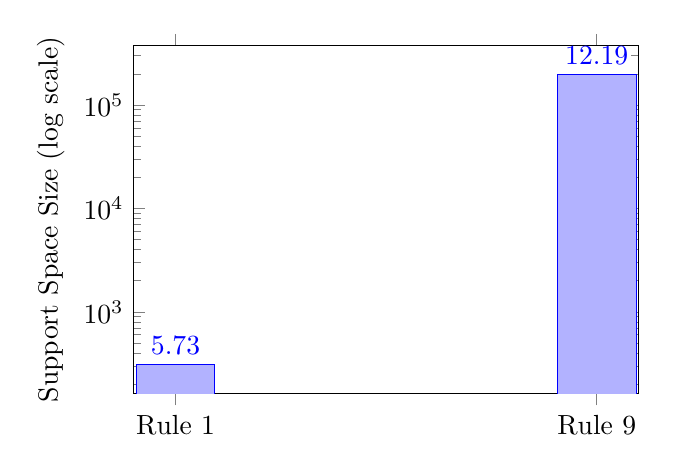
\begin{tikzpicture}
        \begin{axis}[
            ybar,
            bar width=1cm,
            ylabel={Support Space Size (log scale)},
            symbolic x coords={Rule 1, Rule 9},
            xtick=data,
            ymode=log,
            nodes near coords,
            nodes near coords align={vertical},
            width=8cm,
            height=6cm,
        ]
        \addplot coordinates {(Rule 1, 309) (Rule 9, 196524)};
        \end{axis}
    \end{tikzpicture}
    \caption{Support Space Explosion with Irrelevant Predicate (636$\times$ increase)}
\end{figure}

% ----------------------------------------------------------------------------
% SECTION 6: KEY INSIGHTS
% ----------------------------------------------------------------------------
\section{Key Insights}

\subsection{Structural Findings}

\begin{enumerate}
    \item \textbf{High-Quality Compositional Rules}: Transitive rules (grandmother, sibling, aunt) achieve 100\% confidence, indicating a well-structured family knowledge graph.
    
    \item \textbf{Incomplete Inverse Edges}: The Parent/Child inverse rule (83\%) reveals that inverse relations are not always stored bidirectionally.
        
    \item \textbf{Symmetric Relations Work}: Sibling symmetry and gender-specific inverses are fully satisfied.
\end{enumerate}

\subsection{Rule Categories Performance}

\begin{table}[H]
    \centering
    \caption{Rule Type Performance Summary}
    \begin{tabular}{lcc}
        \toprule
        \textbf{Rule Type} & \textbf{Avg Confidence} & \textbf{Assessment} \\
        \midrule
        Transitive/Compositional & 1.0000 & Excellent \\
        Inverse (Symmetric) & 1.0000 & Excellent \\
        Inverse (Parent-Child) & 0.8295 & Incomplete data \\
        \bottomrule
    \end{tabular}
\end{table}

\subsection{Implications for Knowledge Graph Quality}

From our rule mining analysis:

\begin{enumerate}
    \item \textbf{Graph Completeness}: 
    \begin{itemize}
        \item Basic family relations (parent, sibling, grandparent, aunt) are well-populated
    \end{itemize}
    
    \item \textbf{Bidirectionality}:
    \begin{itemize}
        \item Sibling relations are bidirectional
        \item Parent-child relations are partially unidirectional
    \end{itemize}
    
    \item \textbf{Inference Potential}:
    \begin{itemize}
        \item Rules with 100\% confidence can be used for link prediction
        \item Missing grandmother/aunt/sibling edges could be inferred using validated rules
    \end{itemize}
\end{enumerate}

% ----------------------------------------------------------------------------
% SECTION 7: CONCRETE EXAMPLES
% ----------------------------------------------------------------------------
\section{Concrete Examples}

\subsection{Rule 1: Grandmother Logic (Perfect)}

\textbf{Example Match:}
\begin{itemize}
    \item $x$ = claudia814, $y$ = david832, $z$ = isabella815
    \item \texttt{Mother(claudia814, david832)} exists
    \item \texttt{Mother(isabella815, claudia814)} exists
    \item \texttt{Grandmother(isabella815, david832)} exists \checkmark
\end{itemize}

\subsection{Rule 4: Parent/Child Inverse (Exception)}

\textbf{Example Exception:}
\begin{itemize}
    \item $x$ = gabriel708, $y$ = benjamin710
    \item \texttt{Father(gabriel708, benjamin710)} exists
    \item \texttt{Child(benjamin710, gabriel708)} does NOT exist \ding{55}
\end{itemize}

\textbf{Reason}: The inverse \texttt{sonOf} or \texttt{daughterOf} edge was not added to the dataset.

\subsection{Rule 7: First Cousin Once Removed (All Exceptions)}

\textbf{Example Exception:}
\begin{itemize}
    \item $a$ = claudia814, $b$ = david832, $c$ = sofia817, $d$ = natalie838
    \item \texttt{Mother(claudia814, david832)} exists
    \item \texttt{Grandmother(sofia817, claudia814)} exists
    \item \texttt{Daughter(natalie838, sofia817)} exists
    \item \texttt{FirstCousinOnceRemoved(natalie838, david832)} does NOT exist \ding{55}
\end{itemize}

\textbf{Reason}: The \texttt{FirstCousinOnceRemovedOf} relation type for natalie838  and david 832 is incorrect and hence not present in the dataset.

% ----------------------------------------------------------------------------
% SECTION 8: SUMMARY
% ----------------------------------------------------------------------------
\section{Summary}

\subsection{Rules Discovered}

\begin{table}[H]
    \centering
    \caption{Summary of Discovered Rules with High Confidence}
    \begin{tabular}{clc}
        \toprule
        \textbf{ID} & \textbf{Rule} & \textbf{Confidence} \\
        \midrule
        1 & Mother(x,y) $\land$ Mother(z,x) $\rightarrow$ Grandmother(z,y) & 1.00 \\
        2 & Mother(z,x) $\land$ Child(y,z) $\land$ (x$\neq$y) $\rightarrow$ Sibling(x,y) & 1.00 \\
        3 & Mother(x,y) $\land$ Mother(z,x) $\land$ Daughter(w,z) $\rightarrow$ Aunt(w,y) & 1.00 \\
        5 & Sibling(x,y) $\rightarrow$ Sibling(y,x) & 1.00 \\
        6 & SisterOf(x,y) $\land$ isMale(y) $\rightarrow$ BrotherOf(y,x) & 1.00 \\
        \bottomrule
    \end{tabular}
\end{table}

\subsection{Key Results}

\begin{itemize}
    \item \textbf{5 rules with 100\% confidence} (can be used for inference)
    \item \textbf{1 rule with 83\% confidence} (indicates incomplete data)
    \item \textbf{2 rules with 0\% confidence} (missing relation types, semantic mismatch or incorrect rules)
    \item \textbf{Noise analysis}: Irrelevant predicates don't affect confidence but explode search space by 636$\times$
\end{itemize}

\subsection{Output Files}

\begin{itemize}
    \item \texttt{outputs/rules/rule\_metrics.csv} --- Quantitative results
    \item \texttt{outputs/rules/rule\_report.txt} --- Detailed text report
    \item \texttt{outputs/rules/rule\_confidence\_chart.png} --- Confidence visualization
    \item \texttt{outputs/rules/support\_vs\_success.png} --- Support/success scatter plot
    \item \texttt{outputs/rules/noise\_analysis.png} --- Noise experiment visualization
\end{itemize}

% ----------------------------------------------------------------------------
% APPENDIX
% ----------------------------------------------------------------------------
\appendix

\section{Rule Definitions Reference}

\begin{longtable}{cp{10cm}}
    \toprule
    \textbf{ID} & \textbf{Full Definition} \\
    \midrule
    \endhead
    1 & Mother(x, y) $\land$ Mother(z, x) $\rightarrow$ Grandmother(z, y) \\
    2 & Mother(z, x) $\land$ Child(y, z) $\land$ (x $\neq$ y) $\rightarrow$ Sibling(x, y) \\
    3 & Mother(x, y) $\land$ Mother(z, x) $\land$ Daughter(w, z) $\rightarrow$ Aunt(w, y) \\
    4 & Father(x, y) $\rightarrow$ Child(y, x) \\
    5 & Sibling(x, y) $\rightarrow$ Sibling(y, x) \\
    6 & SisterOf(x, y) $\land$ isMale(y) $\rightarrow$ BrotherOf(y, x) \\
    7 & Mother(a, b) $\land$ Grandmother(c, a) $\land$ Daughter(d, c) $\rightarrow$ FirstCousinOnceRemoved(d, b) \\
    8 & Father(a, b) $\land$ FirstCousin(c, a) $\land$ Grandchild(d, c) $\rightarrow$ FirstCousinOnceRemoved(d, b) \\
    9 & Mother(x, y) $\land$ Mother(z, x) $\land$ Sister(a, b) $\rightarrow$ Grandmother(z, y) [Noise Test] \\
    \bottomrule
\end{longtable}

\section{Relation Semantics}

\begin{table}[H]
    \centering
    \caption{Edge Interpretation: (head, tail, relation) means head IS [relation] OF tail}
    \begin{tabular}{ll}
        \toprule
        \textbf{Relation} & \textbf{Meaning} \\
        \midrule
        motherOf & head is the mother of tail \\
        fatherOf & head is the father of tail \\
        sonOf & head is the son of tail \\
        daughterOf & head is the daughter of tail \\
        sisterOf & head is the sister of tail \\
        brotherOf & head is the brother of tail \\
        grandmotherOf & head is the grandmother of tail \\
        grandfatherOf & head is the grandfather of tail \\
        auntOf & head is the aunt of tail \\
        uncleOf & head is the uncle of tail \\
        \bottomrule
    \end{tabular}
\end{table}

\section{Theoretical Background}

\subsection{Rule Mining Algorithms}

Common approaches for automatic rule discovery:
\begin{enumerate}
    \item \textbf{AMIE/AMIE+}: Association rule mining for RDF graphs with PCA confidence
    \item \textbf{AnyBURL}: Anytime bottom-up rule learning
    \item \textbf{RuleN}: Neural rule learning with attention mechanisms
    \item \textbf{NeuralLP}: Differentiable learning of logical rules
\end{enumerate}

\subsection{Confidence Metrics}

\textbf{Standard Confidence:}
\begin{equation}
    \text{conf}(B \Rightarrow H) = \frac{|\{(x,y): B(x,y) \land H(x,y)\}|}{|\{(x,y): B(x,y)\}|}
\end{equation}

\textbf{PCA Confidence} (used in AMIE):
\begin{equation}
    \text{pca\_conf}(B \Rightarrow r(x,y)) = \frac{\text{supp}(B \Rightarrow r(x,y))}{|\{(x,y'): B(x,y') \land \exists y'': r(x,y'')\}|}
\end{equation}

\end{document}
